\documentclass[12pt]{article}
\usepackage{fixltx2e}
\usepackage{tikz}
\usepackage{listings}
\usepackage{graphicx}
\date{}
\title{Assignment - 7}
\begin{document}
\maketitle
\section*{Aim}
8-Queens Matrix is Stored using JSON/XML having first Queen placed, use back-tracking to place remaining Queens to generate final 8-queen's Matrix using Python. Create a backtracking scenario and
use HPC architecture (Preferably BBB) for computation of next placement of a queen.
\section*{Learning Objective}
To understand:
\begin{description}
\item{$\cdot$} Basics of the Backtracking Stratergy for problem solving.
\item{$\cdot$} HPC(High Performance Computing) Architecture.
\item{$\cdot$} Working and implementation of N-Queens problem
\end{description}

\section*{Learning Outcome}
We will be able to
\begin{description}
\item{$\cdot$}Understand the internals of the HPC Architecture by designing the 8-Queens problem using backtracking stratergy.
\end{description}

\section*{Software And Hardware Requirements}
\begin{description}
\item[$\cdot$] Latest 64-BIT Version of Linux Operating System.
\item[$\cdot$] Python Interpreter
\end{description}

\section*{Mathematical Model}
\noindent Let y=f(x) be the solution to the above problem. \\
Let S be a system such that 
S=\{s,e,X,Y,DD,NDD,se,fe,f1,P,sharedMem {\textbar} \o \}
\\
s: Start state of system i.e Y= \o  \\
e:End state of system when i.e. when Y=X \\
X: Set of inputs X=\{$x_1$\}
where 
$x_1$ $\in$ N where N is a even Number $\geq$ 4 \\
\noindent Y: Set of Outputs i.e \{$Y_1$..$Y_n$\} i.e i.e The N-Queens Matrix where $Y_i$=\{$y_1$..$y_n$\}
\noindent f1: Function to Accept Input of N from user \\
\noindent f2: Function to Place Queen \\
\noindent f3: Function to display result of multiplication \\
f3: X$\rightarrow$Y
\noindent se: Success state is when we get correct placement of queens without conflicts \\
fe: Failure State is when we do not get correct placement of queens i.e with conflicts \\
\\
\textbf{Deterministic Data} \\
\\
Value of N\\
\textbf{Non Deterministic Data} \\
Placement of Queens \\
\begin{figure}[ht!]
\centering
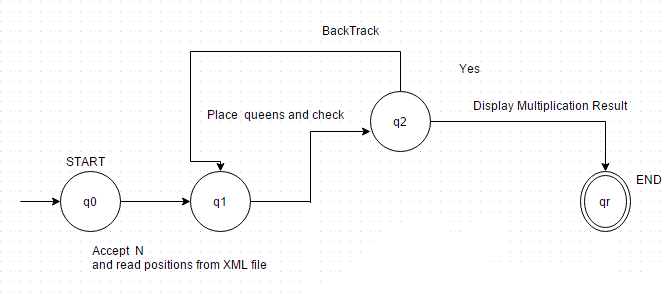
\includegraphics[width=100mm,scale=2]{state7.png}
\caption{State Disagram}
\label{overflow}
\end{figure}
\pagebreak
\section*{UML-CLASS DIAGRAM}
\begin{figure}[ht!]
\centering
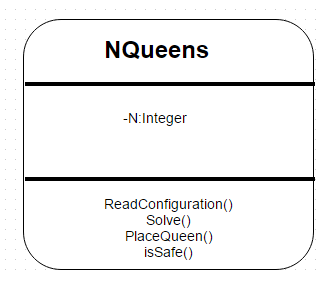
\includegraphics[width=100mm,scale=2]{cd7.png}
\label{overflow}
\end{figure}
\section*{Theory}
\subsection*{N-Queens Problem}
The eight queens problem is the problem of placing eight queens on an 8�8 chessboard such that none of them attack one another (no two are in the same row, column, or diagonal). More generally, the n queens problem places n queens on an n�n chessboard. \\
\subsection*{PsuedoCode}

SolveQueens (Integer boardSize, Queequeen[boardSize]);//
i $\leftarrow$ 0 \\//Begin by placing the queen number 0 \\
while i $\le$  boardSize \\
	queen[i].row <- queen[i].row + 1\\
		//Place queen[i] to next row
	/* If queen[i] exceeds the row count, reset the queen and 
		re-place queen[i-1] \\

	if(queen[i].row $\ge$ boardSize) \\
		queen[i] $\leftarrow$ -1; \\
		i $\leftarrow$ i - 1; \\
	else \\
		//While the queen[i] is under attack move it down the row \\
		while(isUnderAttack(queen[i]) \\
			queen[i].row <- queen[i] + 1; \\
		//if queen[i] exceeds the row count, reset it, re-place queen[i-1] \\
\noindent if(queen[i].row >= boardSize) \\
			queen[i].row $\leftarrow$ -1 \\
			i $\leftarrow$ i - 1; \\
		else \\
			i++; \\
end while \\
		
\subsection*{Backtracking Algorithmic Stratergy}
Backtracking is a general algorithm for finding all (or some) solutions to some computational problems, notably constraint satisfaction problems, that incrementally builds candidates to the solutions, and abandons each partial candidate c ("backtracks") as soon as it determines that c cannot possibly be completed to a valid solution.\\
The classic textbook example of the use of backtracking is the eight queens puzzle, that asks for all arrangements of eight chess queens on a standard chessboard so that no queen attacks any other. In the common backtracking approach, the partial candidates are arrangements of k queens in the first k rows of the board, all in different rows and columns. Any partial solution that contains two mutually attacking queens can be abandoned.\\
Backtracking can be applied only for problems which admit the concept of a "partial candidate solution" and a relatively quick test of whether it can possibly be completed to a valid solution. It is useless, for example, for locating a given value in an unordered table. When it is applicable, however, backtracking is often much faster than brute force enumeration of all complete candidates, since it can eliminate a large number of candidates with a single test.\\
Backtracking is an important tool for solving constraint satisfaction problems, such as crosswords, verbal arithmetic, Sudoku, and many other puzzles. It is often the most convenient (if not the most efficient technique for parsing, for the knapsack problem and other combinatorial optimization problems. 
\subsection*{PsuedoCode}
\textbf{
procedure bt(c) \\
  if reject(P,c) then return \\
  if accept(P,c) then output(P,c) \\
  s ? first(P,c) \\
  while s $\ne$ ? do \\
    bt(s)\\
    s ? next(P,s)\\
    }
\section*{Program Code and Output}
\subsection*{queensserver.py}
\lstinputlisting[language=python,breaklines=true,showspaces=false,showstringspaces = false]{queensserver.py}
\pagebreak
\subsection*{queensclient.py}
\lstinputlisting[language=python,breaklines=true,showspaces=false,showstringspaces = false]{queensclient.py}
\pagebreak

\section*{Result}
Thus,we have designed and implemented Nqueens problem using Backtracking Stratergy in python language and tested the same.
\end{document}